%%%%
% -- Cosmology Science
% --     FOBOS Keck White Paper 2019
%%%%

\begin{figure}[h!]
%
\vskip -0.1in
%
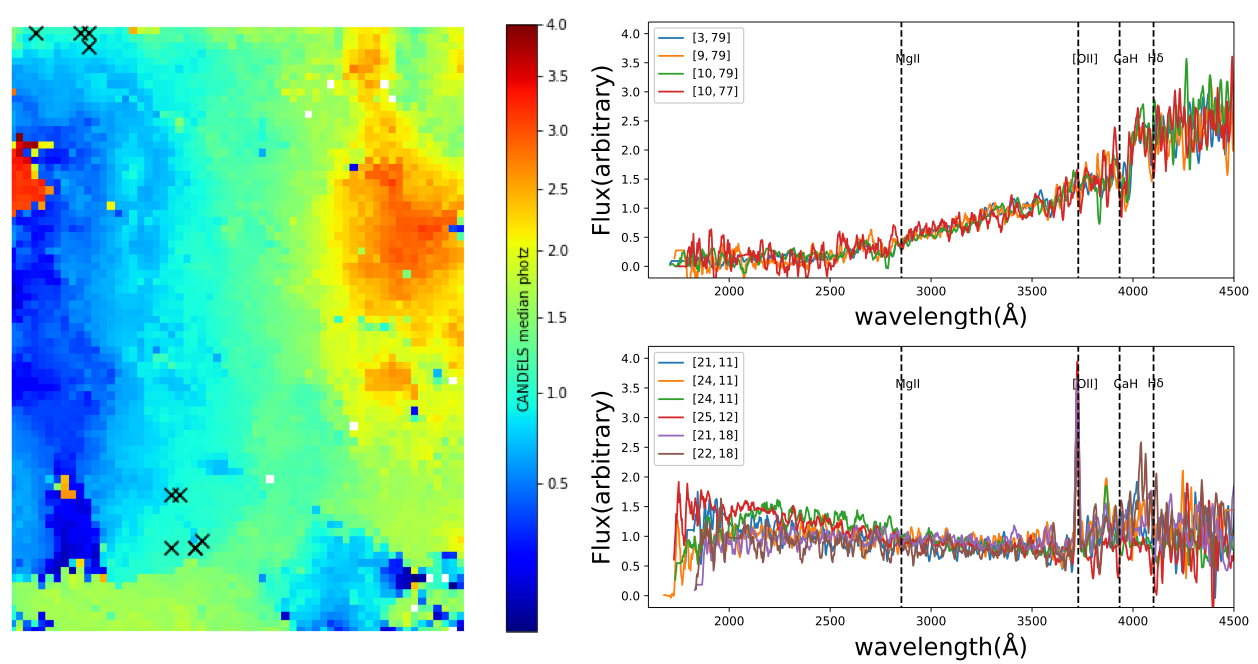
\includegraphics[width=\textwidth]{figs/Hemmati18_Fig8_VVDS_spec.png}
%
\caption{\small {\it Left}: A Self-Organizing Map
\citep[SOM;][]{1990Natur.346...24K} from \citet{hemmati18} encoding the
relation between colors in an LSST+WFIRST-like color space and redshift,
$z$.  Position in the SOM is associated with a position in the
multi-dimensional broad-band color space of galaxies.  Galaxies observed
in this space are assigned $z$ values based on the median photo-$z$ of
galaxies from the CANDELS survey \citep[color
bar;][]{2011ApJS..197...35G}.  Such SOMs can be used to optimally define
spectroscopic training samples for use with imaging surveys.  {\it
Right}: Galaxy spectra from VVDS \citep{2005A&A...439..845L}; black
crosses near the top and bottom of the SOM are plotted in the top and
bottom panels, respectively.  Note the similarity of the high-resolution
spectra associated within the SOM, suggesting that a systematic
spectroscopic exploration of the LSST color space would have
far-reaching benefits to the science return of the mission beyond the
photo-$z$ application.}
%
\label{fig:SOM}
%
\end{figure}

\subsection{Enhancing Dark Energy Probes via Precision Cosmic Distances}
\label{sec:cosmology}

The 2011 Nobel Prize in Physics was awarded for the discovery that the
expansion of the universe is accelerating due to the mysterious ``dark
energy,'' the origin of which remains unknown.  Dark energy is one of
the most fundamental, unsolved problems in both cosmology and particle
physics.  It has inspired enormous world-wide efforts --- culminating in
LSST, Euclid, and WFIRST --- that seek highly precise measures of cosmic
structure to constrain the evolving dark-energy equation-of-state.

These measures utilize angular correlations of galaxy positions, their
gravitational lensing shear, and the cross-correlation between the two.
Unfortunately, photometric distances (via photometric redshifts, or
``photo-$z$s'') are significantly less precise than spectroscopic
redshifts (spec-$z$s), introducing significant biases.  The
spectroscopic validation of photo-$z$s we propose with FOBOS is
therefore critical to the success of {\it all} imaging surveys in this
respect. It would not only \emph{increase the dark energy
figure-of-merit in LSST by 40\%} \citep{newman15} but, importantly,
provide vital confidence in cosmological results.  FOBOS is particularly
powerful in this application because it has no ``redshift desert'' thanks to its unique ability to measure spectroscopic redshifts above $z > 1.5$ via
rest-frame UV features.  This eliminates the need for expensive, space-based\footnote{Ground-based near-IR
spectroscopy is too contaminated by sky-line emission to provide spec-$z$s at the required level of completeness
\citep{newman15}.} near-IR spectroscopy.

\chal{photozs}
%
\begin{enumerate}[rightmargin=0.2cm,leftmargin=0.2cm]
%
\item[] {\textsf {\large Data-Science Challenge \ref{photozs}: Enable
high-precision LSST photometric redshifts with strategically designed
training spectroscopy:}}  FOBOS is ideally suited to obtaining large
($>10,000$ galaxies) and deep spectroscopic training sets required for
LSST, WFIRST, and Euclid \citep[see][] {newman15}.  Applying
machine-learning, template-based, and hybrid photo-$z$ estimators to
simulated data, we will build a methodology for designing FOBOS training
sets that minimize observing time while maintaining adequate
parameter-space sampling.\footnote{
%
Of course, the design of this sample also benefits the data-science
challenges we detail in Section \ref{sec:galaxies}.}
%
Self-Organizing Maps (SOM, Fig.~\ref {fig:SOM}) provide a
state-of-the-art representation of a high-dimensional input space in
projected 2D grid cells, allowing us to benchmark sampling of the
photometric color space under various training set designs.  We will use
Bayesian Optimization techniques to evaluate the success of simulated training sets against the fidelity of full  
cosmological analyses that employ them.  This will enable extremely rapid exploration of the
optimal design space.

\end{enumerate}

%-----------------------------------------------------------------------
\begin{wrapfigure}{r}{0.5\textwidth}\small
%
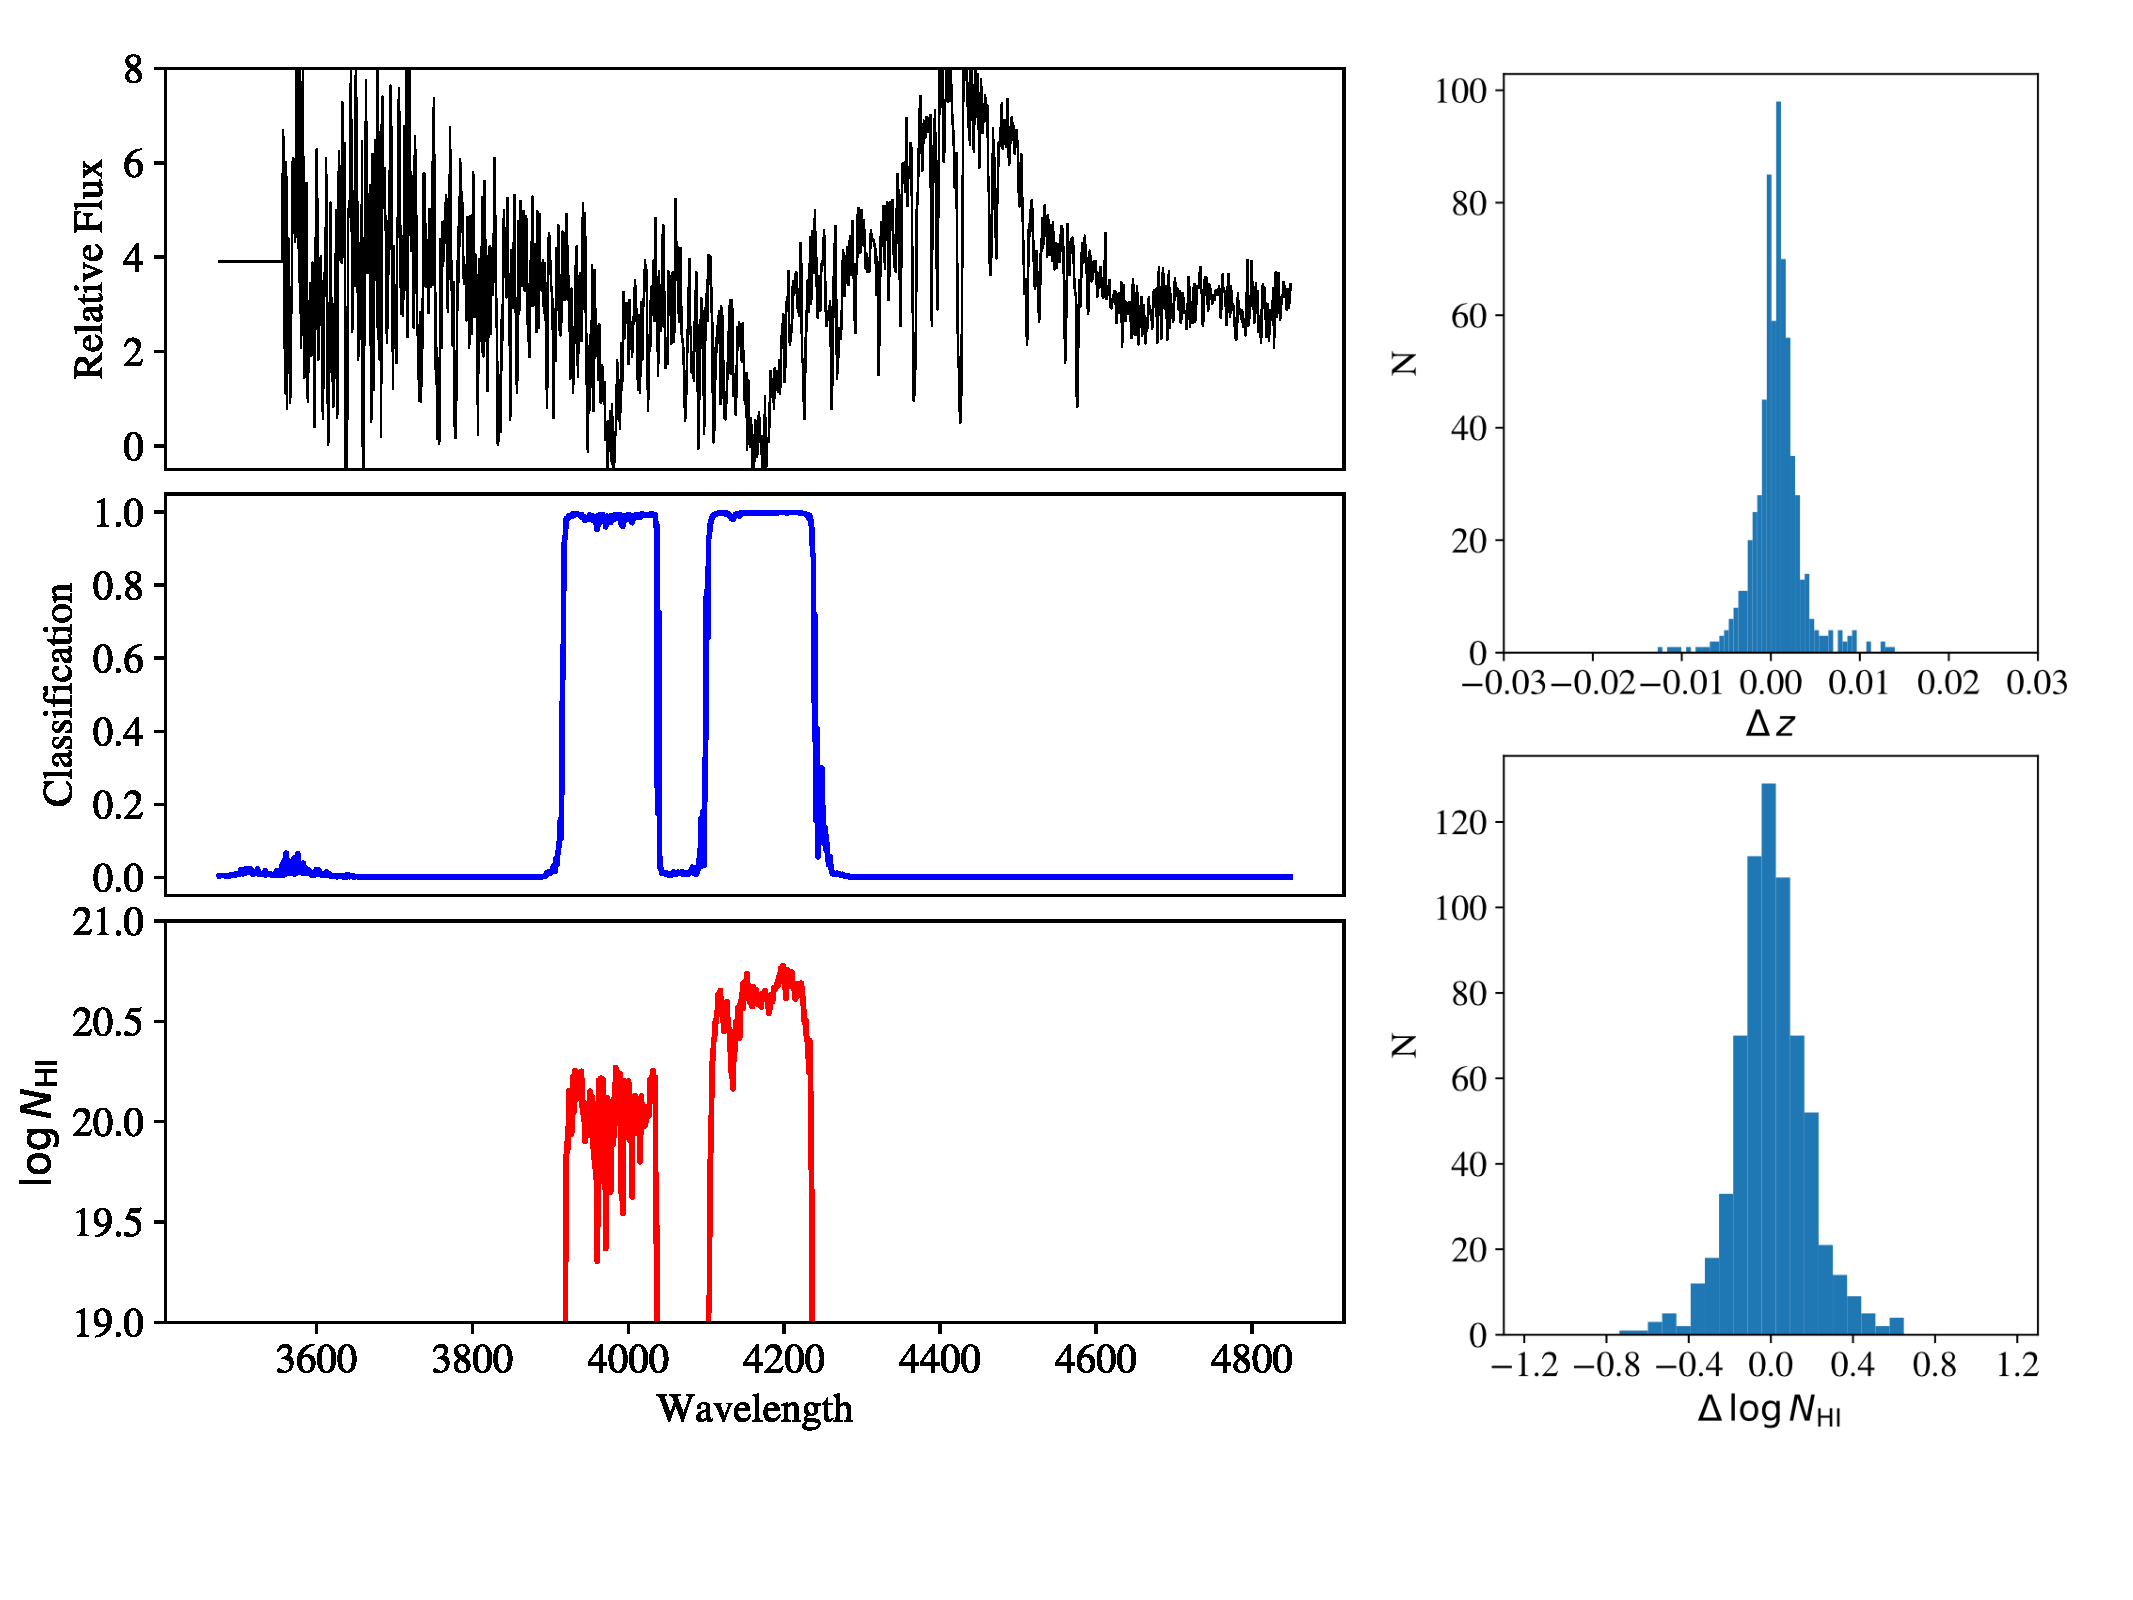
\includegraphics[width=0.5\textwidth]{figs/Parks_fig.pdf}
%
\caption{Application of machine learning to find and quantify the
physical parameters of absorption by neutral hydrogen gas in spectra
taken along quasar sight lines \citep[adapted from Figs 7 and 14
from][]{parks18}.  Two absorption systems in the spectrum (top-left) are
identified (middle-left) and then ``labeled'' with an HI column density
($N_{\rm HI}$) (bottom-left) using a convolutional neural network (CNN).
Redshift, $z$, (top-right) and $N_{\rm HI}$ (bottom-right) measurements
obtained the CNN are in excellent agreement with derivations by experts.
FOBOS will provide rich data sets for similar transfer of
physical parameter labels to photometric and spectroscopic data.}
%
\label{fig:absorber}
%
\end{wrapfigure}